\chapter{Kiến Thức Nền Tảng Và Khảo Sát}
\ifpdf
    \graphicspath{{Chapter2/Chapter2Figs/PNG/}{Chapter2/Chapter2Figs/PDF/}{Chapter2/Chapter2Figs/}}
\else
    \graphicspath{{Chapter2/Chapter2Figs/EPS/}{Chapter2/Chapter2Figs/}}
\fi
\section{Kiến thức nền tảng}
\subsection{Kiến thức về HTML5}
\subsubsection{Tổng quan HTML}
HTML (Hyper Text Markup Language) là ngôn ngữ đánh dấu được sử dụng các thẻ html để biểu diễn nội dung các trang web. Tuy nhiên HTML với riêng nó thì chỉ có thể cung cấp trang tĩnh. Do vậy, để đáp ứng nhu cầu ngày càng tăng, HTML đã kết hợp bổ sung với một số thành phần khác như CSS, Flash,...

HTML ngày nay được gọi là HTML4 được xuất bản lần đầu từ năm 1997. Phiên bản mới nhất của nó chính là HTML4 có từ năm 1999. Vào năm 2000, một ngôn ngữ được gọi là XHTML bắt đầu phát triển và nó được sử dụng trong những năm qua, chủ yếu là do các tiêu chuẩn nghiêm ngặt mà nó đặt ra.

Vấn đề với HTML4 là giới hạn chức năng của nó. Nó phải được mở rộng thông qua các plugin như Flash, cung cấp nhiều hơn so với các văn bản đơn giản và hình ảnh.

Với tất cả những plugin, nó trở nên khó khăn để duy trì các tiêu chuẩn thích hợp. Lý tưởng nhất, tất cả các trình duyệt sẽ hiển thị tất cả các trang web trong cùng một cách để cung cấp những kinh nghiệm tương tự cho mọi người sử dụng. Để hiển thị các kết quả tương tự trên nhiều trình duyệt, các nhà phát triển web cần phải sửa chữa nhanh chóng và thay đổi các thành phần khác nhau trong trang web của họ nhằm thích ứng với quá trình khác nhau. Điều này sẽ trở nên cồng kềnh sau một thời gian áp dụng. Trên một lưu ý thực tế hơn, các trang web yêu cầu plugin như Flash và Java, cuối cùng phải tăng cường hiệu quả bằng cách sử dụng nhiều CPU và RAM trên hệ thống người dùng.

HTML được viết bao gồm các thẻ được đặt trong dấu ngoặc nhọn (như <html>) trong nội dung trang web. Thẻ HTML thường đi theo cặp như <h1> và </h1>, mặc dù một số thẻ không có đi theo cặp như <img>. Thẻ đầu tiên trong một cặp là bắt đầu từ khóa, và thẻ thứ hai là thẻ kết thúc (cũng được gọi là thẻ mở và thẻ đóng). Ở giữa các thẻ có thể thêm văn bản, thẻ, chú thích và các loại nội dung dựa trên văn bản.
Hình thức chung của một phần tử HTML là:

\begin{lstlisting}
	<tag attribute1="value1" attribute2="value2">content</tag>
\end{lstlisting}

Sau đây là ví dụ “Hello World” được thực hiện bằng cách sử dụng 9 dòng mã:

\begin{lstlisting}
  <!DOCTYPE html>
	<html>
   		<head>
     		<title>This is a title</title>
   		</head>
   		<body>
   			<p>Hello World!</p>
   		</body>
 	</html>
\end{lstlisting}


Dòng đầu tiên, <!DOCTYPE html>, là một mô tả về loại tài liệu và nó cho phép trình duyệt biết được về của HTML mà bạn đang sử dụng (trường hợp này là HTML5). Nó rất quan trọng. Nếu không có mô tả này, các trình duyệt sẽ không nhận biết được loại tài liệu và không thể có những thao tác đặc biệt.

Thẻ <html> là thẻ mở và cho trình duyệt biết nội dung giữa nó và thẻ đóng </html> là một tài liệu HTML. Các nội dung giữa cặp <body> và </body> là nội dung chính của tài liệu sẽ xuất hiện trong cửa sổ trình duyệt.


\subsubsection{HTML5}
HTML5 Là phiên bản tiếp sau của HTML 4.01 và XHTML 1.1, HTML5 là một phản ứng để đáp lại lời phê bình rằng HTML và XHTML được sử dụng phổ biến trên World Wide Web là một hỗn hợp các tính năng với các thông số kĩ thuật khác nhau, được giới thiệu bởi nhiều nhà sản xuất phần mềm ví dụ Adobe, Sun Microsystems, Mozilla, Apple, Google,... và có nhiều lỗi cú pháp trong các văn bản web. Đây là một nỗ lực để tạo nên một ngôn ngữ đánh dấu có thể được viết bằng cú pháp HTML hoặc XHTML. Nó bao gồm các mô hình xử lý chi tiết để tăng tính tương thích, mở rộng, cải thiện và hợp lý hóa các đánh dấu có sẵn cho tài liệu, đưa ra các đánh đấu mới và giới thiệu giao diện lập trình ứng dụng (API) để tạo ra các ứng dụng Web phức tạp. Cùng một lý do như vây, HTML5 là một ứng cử viên tiềm năng cho nền tảng ứng dụng di động như điện thoại và máy tính bảng.

HTML5 sẽ là chuẩn mới cho HTML. HTML4 đã làm việc rất tốt, nhưng rõ ràng nó vẫn còn một số nhược điểm.HTML5 được xây dựng trên những nguyên tắc sau đây:

\quad - Ít phụ thuộc vào các chức năng bổ sung.

\quad - Chức năng mới dựa trên HTML, CSS, DOM và JavaScript.

\quad - Script nên được thay thế bằng markup bất cứ khi nào có thể.

\quad - Độc lập thiết bị( tức có sẵn trên tất cả các thiết bị).

\quad - Xử lý lỗi tốt hơn.

\quad - Quá trình phát triển phải được công khai cho mọi người dùng.

\begin{figure}[!h] 
\centering

\includegraphics[scale=0.8]{html5_logo.png}
\caption{Logo HTML5}
\end{figure}

HTML5 là chuẩn mới cho ngôn ngữ đánh dấu (HTML). HTML5 hỗ trợ khắc phục những nhược điểm của phiên bản trước (HTML4) như cần nhiều plug-in để xử lý các nội dung Flash, Silverlight, JavaFX… gây tốn tài nguyên.

Đặc biệt, HTML5 cho biết thêm nhiều tính năng mới. Chúng bao gồm các thẻ mới như <video>, <audio> và <canvas> cũng như tích hợp đồ họa vector SVG (thay thế việc sử dụng thẻ <object>) và MathML cho các công thức toán học. Những tính năng này được thiết kế để làm cho việc xử lý đa phương tiện và đồ họa nội dung trên web dễ dàng hơn mà không cần phải bổ sung các API. Các yếu tố mới khác, chẳng hạn như <section>, <article>, <header> và <nav> được thiết kế để làm phong phú thêm ngữ nghĩa nội dung của tài liệu và thay thế cho sử dụng phổ biến của thẻ <div> và thẻ <span>. Các thuộc tính mới đã được giới thiệu với mục đích tương tự, trong khi một số yếu tố và các thuộc tính đã được loại bỏ. Một số thẻ như <a>, <cite> và <menu> đã được thay đổi, xác định lại hoặc chuẩn hóa. Các API và DOM là bộ phận cơ bản của đặc điểm kỹ thuật HTML5. HTML5 cũng xác định cụ thể một số các xử lý cần thiết cho các tài liệu không hợp lệ để các lỗi cú pháp sẽ được xử lý thống nhất bởi tất cả các trình duyệt phù hợp và các user agents.

HTML5 giới thiệu các yếu tố và các thuộc tính phản ánh việc sử dụng điển hình trên trang web hiện đại. Một số trong số đó là ngữ nghĩa thay thế cho sử dụng phổ biến của khối chung (<div>) và nội tuyến (<span>) các yếu tố, ví dụ <nav> (khối điều hướng trang web), <footer> (thường đề cập đến chân của trang web hoặc dòng cuối cùng của HTML code), hoặc <audio> và <video> thay vì <object>. Một số yếu tố phản đối từ 4,01 HTML đã được giảm xuống, bao gồm các yếu tố thuần túy presentational như <font> và <center>, có ảnh hưởng lâu đã được thay thế bởi nhiều khả năng CSS. Ngoài ra còn có một sự nhấn mạnh đổi mới về tầm quan trọng của DOM scripting (ví dụ, JavaScript) trong hành vi Web.

Cú pháp HTML5 không còn dựa trên SGML mặc dù sự giống nhau của đánh dấu của nó. Nó đã, tuy nhiên, được thiết kế để tương thích ngược với phân tích cú pháp chung của các phiên bản cũ của HTML. Nó đi kèm với một dòng giới thiệu mới giống như một SGML khai báo kiểu tài liệu, <!DOCTYPE html>, mà gây nên các tiêu chuẩn phù hợp chế độ dựng hình. Tính đến ngày 5 tháng 1 năm 2009, HTML5 cũng bao gồm hình thức Web 2.0, một riêng biệt với đặc điểm kỹ thuật WHATWG trước đây.

Ngoài ra, HTML5 còn cung cấp:

\quad - Các thẻ mô tả chính xác những gì chúng được thiết kế để chứa đựng.

\quad - Tăng cường khả năng truyền thông trên mạng.

\quad - Chế độ làm việc ngoại tuyến cho ứng dụng web.

\quad - Thao tác kéo thả.

\quad - Cải thiện khả năng lưu trữ chung.

\quad - Các trình làm việc trên nền Web (Web Workers) để chạy các quá trình nền.

\quad - Giao diện WebSocket để thiết lập kết nối liên tục giữa các ứng dụng cư trú và máy chủ.

\quad - Truy vấn dữ liệu đã được lưu trữ tốt hơn.

\quad - Cải thiện tốc độ nạp và lưu trang.

\quad - Hỗ trợ cho CSS3 để quản lý giao diện người dùng đồ họa (GUI), có nghĩa là HTML5 có thể được định hướng nội dung.

\quad - Cải thiện xử lý biểu mẫu trình duyệt.

\quad - Một API cơ sở dữ liệu dựa trên SQL cho phép lưu trữ cục bộ, phía máy khách..

\quad - Canvas và video, để thêm đồ họa và video mà không cần cài đặt các plug-in của bên thứ ba.

\quad - Đặc tả Geolocation API (API định vị toàn cầu), sử dụng khả năng định vị của máy điện thoại thông minh để kết hợp các dịch vụ và các ứng dụng đám mây di động.

\quad - Các biểu mẫu cải tiến làm giảm nhu cầu phải tải về mã JavaScript, cho phép truyền thông hiệu quả hơn giữa các thiết bị di động và các máy chủ điện toán đám mây.

\subsubsection{HTML5 trong thiết bị di động}

Trong các thiết bị di động, HTML5 thường được sử dụng cho các trang web điện thoại di động và các ứng dụng di động trên các hệ điều hành di động như Firefox OS, Tizen, và Ubuntu Touch. Nó cung cấp các nhà phát triển với các công cụ như Offline Web Storage, GeoLocatịon API, Canvas, CSS3, và nhiều hơn nữa.

Trong Windows 8 và Windows Phone 8, các nhà phát triển có thể xây dựng ứng dụng HTML5 kiểu Modern UI.

\begin{figure}[!htb] 
\centering
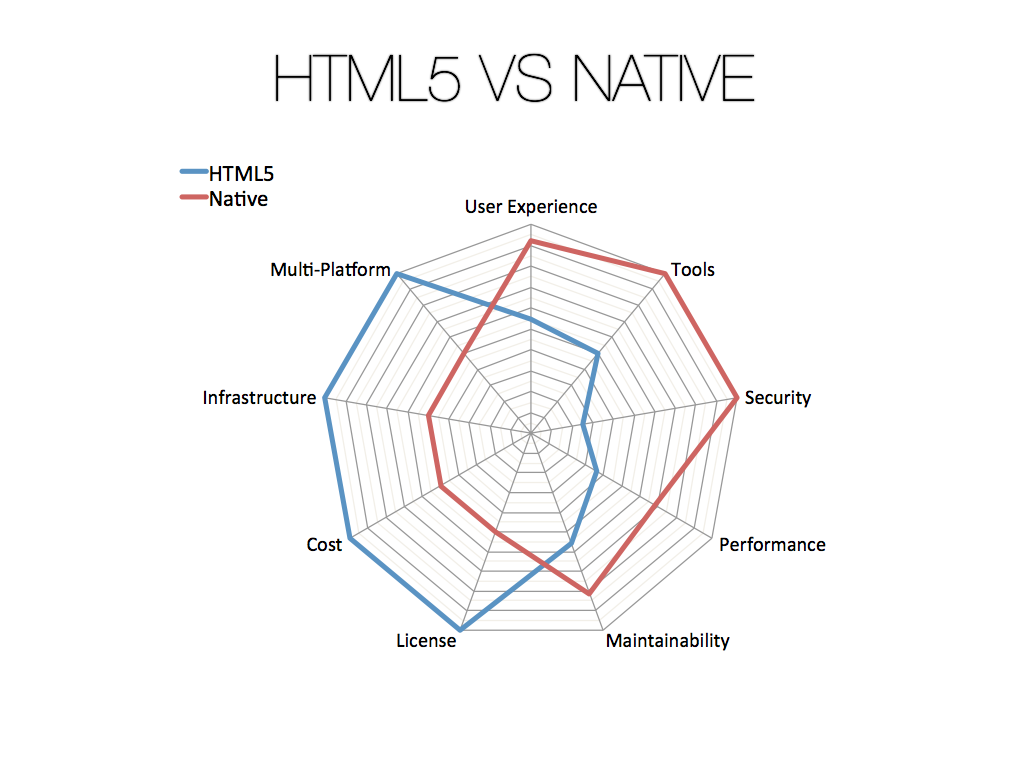
\includegraphics[scale=0.4]{html5_mobile.png}
\caption{HTML5 vs NATIVE }
\end{figure}

Các tính năng chính hỗ trợ cho các thiết bị di động

\textbf{Hỗ trợ offline:}

Các AppCache và cơ sở dữ liệu làm cho nó có thể cho các nhà phát triển di động để lưu trữ những thứ trên các thiết bị và gián đoạn trong kết nối sẽ không ảnh hưởng đến khả năng cho một người nào đó để có được công việc của họ thực hiện.

Hỗ trợ offline giúp trình duyệt bộ nhớ cache các trang tĩnh. Họ phụ thuộc nhiều vào HTTP tiêu đề phản ứng gửi bởi máy chủ web để lấy HTML, CSS và đa phương tiện cần thiết để làm cho trang web. Nếu tất cả mọi thứ cần thiết để làm được lưu trữ, sau đó sẽ được tải nhanh chóng, nhưng ngay cả khi một mục không được lưu trữ sau đó tất cả mọi thứ chậm lại đáng kể.

Để cung cấp hỗ trợ offline, một biểu hiện tập tin bộ nhớ cache phải được tạo ra để xác định ứng dụng của tài nguyên ẩn-tức là các trang của nó, hình ảnh, và các tập tin khác cần thiết để chạy offline. Thông thường, các biểu hiện cũng có một ý kiến được thay đổi khi có các nguồn tài nguyên thay đổi, khiến trình duyệt để làm mới bộ nhớ cache.

\textbf{Canvas:}

Các trang web có thể đánh dấu ra một không gian trên một trang mà hình ảnh tương tác, biểu đồ và đồ thị, các thành phần trò chơi, và tưởng tượng khác có thể được rút ra trực tiếp bằng mã lập trình và tương tác người dùng - không có flash hoặc các plug-in được yêu cầu.

\textbf{Video và hỗ trợ truyền audio:}

Phát triển đang trong giai đoạn rất sớm và phải gián đoạn định dạng, nhưng các trang web như YouTube và Pandora một ngày có thể bỏ qua flash hoàn toàn và mang lại chức năng phát lại theo thời gian và các tính năng hơn nữa.

\textbf{GeoLocation API:}

Điều này thực sự không phải một phần của HTML5, nhưng là một đặc điểm kỹ thuật riêng biệt. Các định vị API cho phép bạn chia sẻ vị trí của bạn với các trang web đáng tin cậy. (Điều này thực sự là vị trí địa lý của thiết bị hoặc kết nối internet của bạn, quyết định dựa trên sự kết hợp của GPS, gia tốc, điện thoại di động tháp tam giác, và ISP hồ sơ địa chỉ.) Các vĩ độ và kinh độ có sẵn để JavaScript trên trang web, mà trong lần lượt có thể gửi lại cho máy chủ web từ xa và cho bạn nhận biết vị trí nội dung như các doanh nghiệp địa phương hoặc hiển thị vị trí của bạn trên bản đồ.
Sau đây là nổi bật API cho một định vị.
 navigator.geolocation.getCurrentPosition(successCallback, errorCallback, options);
Định vị là một đối tượng mà là một phần của đối tượng Navigator. Nó sử dụng phương thức getCurrentPosition(). Tìm kiếm vị trí là một hoạt động không đồng bộ vì nó đòi hỏi sự cho phép của người dùng để truy cập. Do đó chức năng gọi lại cho sự thành công và thất bại là bắt buộc.

\textbf{Form nâng cao:}

Ngay cả điều đơn giản như những cải tiến trong HTML5 cho các hình thức có thể làm cho cuộc sống dễ dàng hơn cho các ứng dụng điện thoại di động. Các lĩnh vực có thể được xác nhận bởi các trình duyệt được cải tiến cho các thiết bị di động. Các chi tiết mà có thể được xử lý bởi các trình duyệt có nghĩa là ít thời gian tải JavaScript mã và các chuyến đi vòng ít đến máy chủ nếu xác nhận có thể được tìm thấy trước khi biểu mẫu được đăng.

\subsection{Kiến thức về JavaScript}
\subsubsection{Tổng quan về JavaScript}
JavaScript là một ngôn ngữ lập trình. Là một phần của các trình duyệt web, cho phép triển khai kịch bản phía máy khách để tương tác với người sử dụng, kiểm soát trình duyệt, giao tiếp không đồng bộ, và làm thay đổi nội dung được hiển thị. Nó cũng đã trở nên phổ biến trong lập trình phía máy chủ, phát triển trò chơi và tạo ra các ứng dụng máy tính.

JavaScript có cú pháp bị ảnh hưởng bởi C cũng như có nhiều quy ước đặt tên từ Java, nhưng chúng không liên quan và có ngữ nghĩa rất khác nhau. Đây là một mô hình đa ngôn ngữ, hỗ trợ hướng đối tượng, bắt buộc, và mang phong cách lập trình chức năng.
 
Là ngôn ngữ thông dịch, đoạn mã JavaScript được nhúng hoặc tích hợp vào file HTML. Khi trang web được tải trong trình duyệt hỗ trợ JavaScript, Trình duyệt sẽ thông dịch và thực hiện các lệnh JavaScript.

JavaScript được sử dụng nhằm bổ sung sự tương tác cho các trang HTML như:

\quad - JavaScript có thể đáp ứng các sự kiện như tải hay loại bỏ các form. Khả năng này cho phép JavaScript trở thành một ngôn ngữ script động.

\quad - JavaScript có thể được sử dụng để xác nhận dữ liệu người dùng nhập vào trước khi nó được chuyển đến server.

\quad - Sử dụng JavaScript có thể giúp website của bạn tương tác với người dùng 1 cách uyển chuyển hơn.

\quad - Tùy biến trình duyệt...

Tóm lại, JavaScript giống như phần hồn của một trang web, giúp người sử dụng có thể tương tác một cách tiện lợi hơn bên cạnh phần xác HTML.


\subsubsection{Cấu trúc và các thành phần trong JavaScript}
\textbf{Các kiểu dữ liệu}

Một biến trong JavaScript các kiểu dữ liệu. Ba kiểu thông thường là: boolean, number, string. Hai kiểu phức tạp là: array và object. Và cuối cùng là kiểu đặc biệt: NULL.

\textbf{Biến}

Biến trong JavaScript đuợc khai báo bởi từ khóa “var” và theo sau là tên của biến. Tên biến phân biệt chữ hoa và chữ thường. Tên biến phải bắt dầu bằng một chữ cái hay một dấu gạch nối, theo sau là các chữ cái, chữ số hay là dấu gạch nối. Thậm chí ta cũng không cần khai báo từ khóa "var" nhưng điều này không được khuyến cáo sử dụng.
  
Ví dụ:  
\begin{lstlisting}
	var name1="John";
	var name2="John";
	name3="John";
\end{lstlisting}


\textbf{Cấu trúc rẽ nhánh}

Các câu lệnh này cho phép chúng ta phân biệt các khối mã lệnh mà sẽ được thực thi chỉ khi gặp phải các điệu kiện nào đó. JavaScript cung cấp hai cấu trúc lệnh điều kiện. Đầu tiên là if...else, cho phép chúng ta có thể kiểm tra một số lượng các biểu thức và thực thi các câu lệnh theo giá trị của chúng. Nếu chúng ta mong muốn kiểm tra một biểu thức đơn lẻ với một số lượng các giá trị, JavaScript cũng cung cấp một cấu trúc switch...case mà có thể làm đơn giản hoá đi phép toán này.
 
Câu lệnh “if… else…”: Câu lệnh if là một trong những đặc tính quan trọng nhất của mỗi  ngôn ngữ lập trình. Nó cho phép thực thi chọn lựa các dòng mã lệnh chỉ khi thoả mãn các điều kiện cụ thể.
  
Câu lệnh “switch… case…”: được sử dụng khi một biến riêng rẽ đang được kiểm tra so với các giá trị khác.Ví dụ:

\begin{lstlisting}
switch (country) { 
       case "ca": 
          alert ("Canada"); 
          break; 
       case "uk": 
         alert ("the United Kingdom"); 
          break; 
       default:  
          alert ("the United States"); 
}
\end{lstlisting}


Khi câu lệnh switch thực hiện kiểm tra giá trị của biến country và so sánh nó với mỗi một trong các giá trị trong các mệnh đề case. Khi một giá trị thích hợp được tìm thấy, các câu lệnh kết hợp với case được thực hiện cho đến khi gặp câu lệnh break. Còn nếu không tìm ra được giá trị thích hợp nào thì câu lệnh default sẽ được thực hiện.

\textbf{Vòng lặp}  

Các vòng lặp chính là các phương tiện của việc thực thi một khối mã lệnh trong một số lần cho trước hay là cho đến khi gặp phải một điều kiện nhất định. 
JavaScript có hai loại vòng lặp: vòng lặp while kiểm tra điều kiện trước hay là sau mỗi bước tính lặp đi lặp lại và thực hiện lặp lại chỉ khi điều kiện là đúng. Một kiểu lặp khác là for, trong trường hợp này, số lượng bước tính lặp đi lặp lại được qui định trước khi lặp lần đầu và không thể bị thay đổi.  
Vòng lặp while: là câu lệnh lặp đơn giản nhất. Cú pháp tương tự như câu lệnh if:

\begin{lstlisting}
	while (i < 10) {
	    alert(i);
	    i = i + 1;
	}
\end{lstlisting} 

Vòng lặp for: Cấu trúc của vòng lặp for là khá phức tạp hơn mặc dù vòng lặp for thường tiện lợi hơn vòng lặp while:

\begin{lstlisting}
	for (var i = 1; i < 10; i++) {
	    alert(i);
	}
\end{lstlisting}


\textbf{Hàm}

Tên hàm có thể được gọi tại bất kỳ đâu trong chương trình, cho phép các đoạn mã thể hiện bởi tên của nó được thực hiện lặp lại khi cần thiết. Tạo một hàm JavaScript là một quá trình đơn giản. Bạn có thể tạo một hàm tại bất kỳ nơi nào trong chương trình JavaScript. Tuy nhiên, cho mục đích tổ chức bạn có thể thấy rằng sự thuận lợi khi đặt tất cả các hàm được dự định sẽ sử dụng trong script tại đầu mỗi file script. Một phương thức khác cho việc tổ chức hàm mà có thể giảm đi sự dư thừa đáng kể và tăng việc sử dụng lại là đặt các hàm trong những file riêng rẽ (được xem như là một thư viện).
    
Ví dụ khai báo một hàm sau:  

\begin{lstlisting}
	var add = function (a, b) { return a + b; }; 
\end{lstlisting}

Ta có thể lưu các hàm như giá trị của một biến, và gọi một hàm bằng cách sử dụng biến này và một cặp dấu ngoặc đơn. Điều này cũng được gọi là gọi hàm.

\subsubsection{DOM}

Document Object Model là một cách để thao tác các cấu trúc và phong cách của một trang HTML. Nó đại diện cho phần bên trong của các trang như cách trình duyệt nhìn thấy nó, và cho phép các nhà phát triển để thay đổi nó với JavaScript.

HTML là một cấu trúc XML giống như trong các yếu tố tạo thành một cấu trúc của nút cha với nút con, như các nhánh của một cây. Có một phần tử gốc (<html>) với các nhánh như <head> và <body>. Vì lý do này, DOM cũng được gọi là cây DOM.

Sửa đổi DOM, bằng cách chọn một phần tử và thay đổi một thuộc tính về nó, là một việc thực hiện thường xuyên trong JavaScript. Để truy cập vào DOM từ JavaScript, sử dụng các đối tượng document. Nó được cung cấp bởi các trình duyệt và cho phép mã trên trang để tương tác với các nội dung.

Điều đầu tiên phải biết là làm thế nào để có được một phần tử. Có một số cách để làm việc đó, và các trình duyệt hỗ trợ những người khác nhau. Cách hay sử dụng nhất là chọn đối tượng theo ID riêng biệt của đối tượng đó.

\begin{lstlisting}
	var pageHeader = document.getElementById('page-header');
\end{lstlisting}

Các đối tượng có “id=pageHeader” sau đó có thể được thao tác. Các thuộc tính của nó có thể được thay đổi, và mã khác có thể được khai báo để xử lý các yếu tố được click hoặc hover.


\subsubsection{Sự kiện(event)}

Trong trình duyệt nhất đang hướng sự kiện và viết các ứng dụng tương tác trong JavaScript thường là về chờ đợi và phản ứng với các sự kiện để thay đổi hành vi của trình duyệt một cách nào đó. Sự kiện xảy ra khi tải trang, khi có tương tác người dùng (click, hover, change…). Dưới đây là một nhóm trong những điều cần thiết để lắng nghe cho một sự kiện, chức năng gọi lại, một phần tử gọi đến một sự kiện:
 
\begin{lstlisting}
	var handleClick = function (event) { // do something! }; 
	var button = document.querySelector('#big-button'); 
	button.addEventListener('click', handleClick);
\end{lstlisting}


addEventListener() là một phương thức được tìm thấy trên tất cả các yếu tố DOM. Ở đây nó được gọi là trên một phần tử được lưu trong biến button. Tham số đầu tiên là một chuỗi - tên của sự kiện để lắng nghe. Dưới đây là đó là click – sự kiện nhấp chuột. Thứ hai là chức năng callback – ở đây gọi hàm handleClick.
Có nhiều loại sự kiện mà JavaScript hỗ trợ và được sử dụng phổ biến như onblur, onchange, onsubmit, onkeydown, onmouseover…

\subsubsection{AJAX}

Để có được nội dung mới của trang web, ta phải di chuyển từ trang này sang trang kế tiếp. Nhưng như các nhà phát triển có nhiều tham vọng hơn với các trang web, cố gắng để xây dựng tương tác thật nhất, và rõ ràng là cần thiết để có thể là một cách để tải nội dung mới vào một trang mà không cần tải lại đầy đủ.

Để tải nội dung mới cho một trang, như nội dung mới trên một trang web hoặc thông báo có email mới, một công cụ được gọi là một yêu cầu XML HTTP (XHR) được sử dụng. Các ứng dụng web mà làm điều này còn được gọi là các ứng dụng AJAX. AJAX là viết tắt của Asynchronous JavaScript And XML.

\begin{figure}[!htb] 
\centering
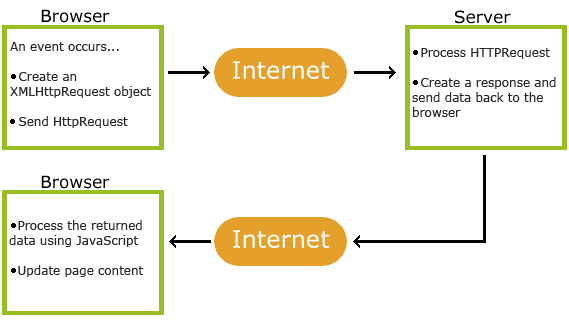
\includegraphics[scale=0.8]{ajax.png}
\caption{Công nghệ AJAX}
\end{figure}

Ví dụ về một XMLHttpRequest:

\begin{lstlisting}
var req = new XMLHttpRequest(); 
req.onload = function (event) { . . . }; 
req.open('get', 'some-file.txt', true); 
req.send(); 
\end{lstlisting}

Điều đầu tiên là tạo mới một XMLHttpRequest bằng cách sử dụng từ khóa “new”, và gọi XMLHttpRequest như một hàm.
Sau đó, chỉ định một hàm callback, để được gọi khi dữ liệu được nạp. Nó được thông qua thông tin về sự kiện này như là đối số đầu tiên.

Sau đó, xác định như thế nào để có được những dữ liệu bằng cách sử dụng req.open. Tham số đầu tiên là phương pháp HTTP (GET, POST, PUT vv). Tiếp theo là các URL để lấy từ dữ liệu (tương tự như href thuộc tính của một liên kết).

Tham số thứ ba là một biến boolean xác định xem yêu cầu là không đồng bộ - ở đây là true, vì vậy XMLHttpRequest được gửi và sau đó thực thi mã vẫn tiếp tục cho đến khi một phản hồi từ máy chủ làm cho hàm onload được gọi lại.

Giá trị mặc định tham số không đồng bộ là false, tức là thực hiện của mã này sẽ tạm dừng tại dòng này cho đến khi dữ liệu được lấy ra và yêu cầu được gọi là đồng bộ. XMLHttpRequests đồng bộ không được sử dụng thường xuyên như là một yêu cầu tới một máy chủ được gửi đi liên tục.

Trên dòng cuối cùng chúng em cho trình duyệt để gửi đi các yêu cầu dữ liệu.

\subsubsection{LocalStorage}

\textbf{LocalStorage}
Khi xây dựng các ứng dụng JavaScript phức tạp chạy trong trình duyệt của người dùng nó rất hữu ích để có thể lưu trữ thông tin trong trình duyệt, do đó các thông tin có thể được chia sẻ trên các trang khác nhau và các phiên duyệt web.
Trong thời gian qua điều này sẽ chỉ thực hiện được với các tập tin cookie - tập tin văn bản được lưu vào máy tính của người dùng - nhưng cách quản lý những việc này với JavaScript là không tốt. Bây giờ có một công nghệ mới được gọi là LocalStorage mà không một điều tương tự, nhưng với một giao diện dễ dàng hơn để sử dụng.

Không giống như các tập tin cookie, Local Storage chỉ có thể được đọc phía máy khách - đó là, bởi trình duyệt và JavaScript. Nếu muốn chia sẻ một số dữ liệu với máy chủ, các tập tin cookie có thể là một lựa chọn tốt hơn.
Để lưu dữ liệu, sử dụng localStorage.getItem:
localStorage.setItem('name', 'tom'); 
Đối số đầu tiên xác định tên sẽ sử dụng để lấy dữ liệu ra. Đối số thứ hai là các dữ liệu ta muốn lưu trữ.
Nhận được trở lại một lần nữa là rất đơn giản - chỉ cần gọi phương thức localStorage.getItem
var name = localStorage.getItem('name');


\textbf{SessionStorage}

Chức năng tương tự như LocalStorage, tuy nhiên dữ liệu sẽ được xóa khi thoát khỏi trình duyệt, hay ứng dụng do đó không gây tốn kém tài nguyên và bảo mật dữ liệu hơn.


\subsubsection{Thư viện Jquery}

jQuery là thư viện JavaScript đa trình duyệt được thiết kế để đơn giản hóa lập trình phía máy người dùng của HTML. jQuery được làm cho việc di chuyển một tài liệu dễ dàng hơn, chọn các yếu tố DOM, tạo ra hiệu ứng, xử lý sự kiện, và phát triển ứng dụng AJAX.

\textbf{Cách sử dụng jQuery}

jQuery thay đổi cách chọn một đối tượng DOM, khiến cho việc thao tác với đối tượng trở nên đơn giản hơn. Thay vì sử dụng phương thức getElementsById(id) của JavaScript thuần, jQuery thu gọn lại bằng cách viết \textdollar(id).

Ví dụ:

\begin{lstlisting}
//trong JavaScript
document.getElementsById("header")[0].innerHTML = "Change the page.";
//trong Jquery
$("#header").html("Change the page.");
\end{lstlisting}

\textbf{AJAX}

jQuery có thể thực hiện trình duyệt độc lập truy vấn AJAX sử dụng cú pháp \textdollar.ajax đơn giản hơn và phương pháp liên kết để tải và thao tác dữ liệu từ xa.

\begin{lstlisting}
$.ajax ( {
   type : "POST" ,
   url : "example.php" ,
   data : "name=John&location=Boston"
 } ) . done ( function ( msg ) {
   alert ( "Data Saved: " + msg ) ;
 } ) . fail ( function ( xmlHttpRequest , statusText , errorThrown ) {
   alert (
     "Your form submission failed. \n \n "
       + "XML Http Request: " + JSON. stringify ( xmlHttpRequest )
       + ", \n Status Text: " + statusText
       + ", \n Error Thrown: " + errorThrown ) ;
 } ) ;
\end{lstlisting}

\subsubsection{Thư viện Jquery Mobile}

jQuery Mobile là một framework web được tối ưu cho màn hình cảm ứng (được gọi là một thư viện JavaScript hoặc một framework di động) hiện đang được phát triển bởi nhóm dự án jQuery. Sự phát triển tập trung vào việc tạo ra một khuôn khổ tương thích với một loạt các điện thoại thông minh và máy tính bảng. jQuery Mobile là tương thích với các framework ứng dụng di động và các nền tảng khác như như PhoneGap, Worklight và nhiều hơn nữa.

Tính năng:

\quad - Tương thích với tất cả các nền tảng di động lớn cũng như tất cả các trình duyệt máy tính để bàn lớn, bao gồm iOS, Android, Blackberry, WebOS, Symbian, Windows Phone và nhiều hơn nữa.

\quad - Được xây dựng trên lõi jQuery vì vậy nó khá quen thuộc cho những người đã biết cú pháp jQuery.

\quad - Cho phép tạo ra các chủ đề, giao diện tùy chỉnh.

\quad - Hạn chế phụ thuộc và nhẹ để tối ưu hóa tốc độ.

\quad - Codebase cơ bản giống nhau sẽ tự động quy mô cho bất kỳ màn hình.

\quad - Cấu hình hướng HTML5 để đặt ra các trang web có đoạn mã tối thiểu.

\quad - Hướng Ajax hỗ trợ với quá trình hiệu ứng chuyển đổi trang, cung cấp khả năng làm sạch các URL thông qua pushState.

\quad - Vật dụng giao diện người dùng tối ưu hóa cảm ứng.

Một trang web sử dụng jQuery Mobile thường có một "header", một "footer" và "content”. Một file HTML có thể chứa nhiều hơn một yếu tố "page" do đó nhiều hơn một "trang web". Bằng cách này, nó chỉ là cần thiết để tải một tập tin bao gồm nhiều trang. Một trang có thể liên kết đến một trang khác trong cùng một tập tin bằng cách sử dụng "\#" cùng với id của nó (ví dụ: href = “\#second”).

Ngoài ra, jQuery Mobile còn có các thuộc tính “data-” với các chức năng khác nhau:

\quad -vData-role: Xác định vai trò của các yếu tố, như tiêu đề, nội dung, footer,…

\quad - Data-position: xác định xem thành phần sẽ được cố định, trong trường hợp này nó sẽ làm cho đối tượng ở phía trên (đối với header) hoặc dưới (đối với footer).

\quad - Data-transition: mô tả quá trình chuyển đổi để sử dụng khi tải trang mới, có thể được thiết lập để: slide, slideUp, slideDown, pop, slide hoặc fade…

\quad - Data-theme: mô tả chủ đề thiết kế để sử dụng cho các yếu tố bên trong container, có thể được thiết lập để chọn các giao diện có sẵn.

Ví dụ:

\begin{lstlisting}
<div data-role="header" data-theme="b"> 
	<h1>Page Title</h1> 
</div>
\end{lstlisting}

Đoạn mã trên đã đặt thẻ “div” ở vị trí đầu trang (header) và qua định giao diện có sẵn “b” của jQuery Mobile.

\subsubsection{Ghi chú quan trọng cần nhớ khi sử dụng JavaScript}

Lệnh Javascript phân biệt chữ in hoa và chữ thường.

Mội câu lệnh Javascript đều kết thúc bằng dấu chấm phẩy “;”.

Các điều kiện phải được khai báo trong cặp dấu ngoặc đơn ().

Khi sử dụng lệnh điều khiển, nếu sử dụng nhiều hơn 1 lệnh, phải sử dụng cặp dấu ngoặc nhọn {}

Javascript sử dụng dấu chấm “.” để tham chiếu đến 1 phương thức hay thuộc tính của đối tượng 

\subsection{Hệ thống quản lý học tập Moodle}

Moodle (viết tắt của Modular Object-Oriented Dynamic Learning Environment) là một nền tảng phần mềm miễn phí về e-learning, còn được gọi là một hệ thống quản lý học tập (Learning Management System). Moodle được phát triển để giúp các nhà giáo dục tạo ra các khóa học trực tuyến tập trung vào sự tương tác và xây dựng hợp tác nội dung, và đang trong quá trình tiến hóa liên tục.

Moodle cho phép tạo các khóa học trên Internet hay các trang web học tập trực tuyến. Moodle được thiết kế dựa trên module nên ta có thể chỉnh sửa giao diện bằng các theme có sẵn hoặc thêm một theme mới cho riêng mình.

\begin{figure}[!htb] 
\centering
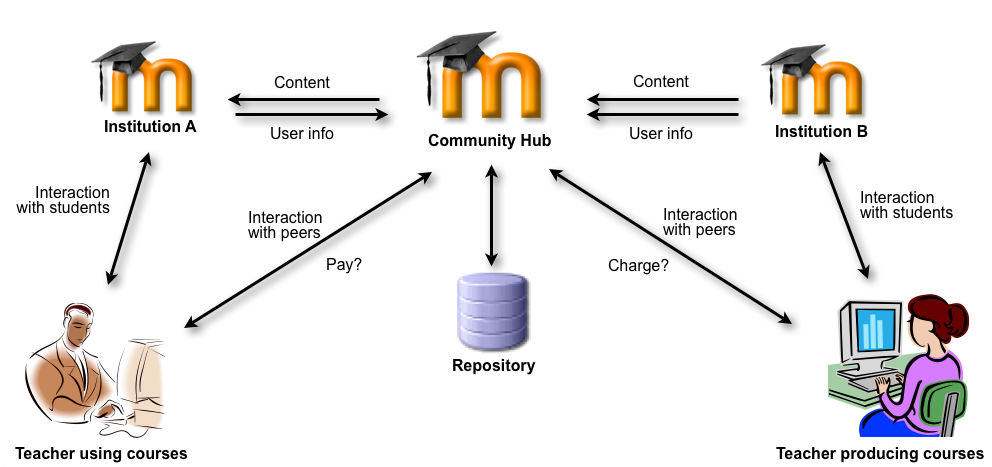
\includegraphics[scale=0.4]{moodle_system.png}
\caption{Moodle}
\end{figure}

Moodle hoàn toàn phù hợp với nhiều cấp học và loại hình đào tạo như phổ thông, đại học hoặc cao đẳng, chính quy hoặc không chính quy và trong các tổ chức, công ty.
Moodle được phát triển dựa trên PHP, có thể triển khai trên một nhóm nhỏ hoặc trên cả các cụm đại học lớn. Vì thế, Moodle có thể giúp chúng ta tiết kiệm rất nhiều khi triển khai một hệ thống e-Learning.
Một số tính năng điển hình của Moodle là:

\quad - Trình chuyển nhượng

\quad - Diễn đàn thảo luận

\quad - Các tập tin tải về

\quad - Phân loại

\quad - Tin nhắn tức thời moodle

\quad - Lịch trực tuyến

\quad - Tin tức trực tuyến và thông báo

\quad - Bài kiểm tra trực tuyến

\quad - Wiki

Phát triển có thể mở rộng xây dựng mô-đun của Moodle bằng cách tạo bổ sung cho chức năng mới cụ thể. Cơ sở hạ tầng của Moodle hỗ trợ nhiều loại plug-in :

\quad - Hoạt động (bao gồm cả chữ và các trò chơi toán học)

\quad - Các loại tài nguyên

\quad - Dạng câu hỏi (nhiều lựa chọn, đúng và sai, điền vào chỗ trống, vv)

\quad - Kiểu trường dữ liệu (đối với hoạt động cơ sở dữ liệu)

\quad - Giao diện đồ họa

\quad - Phương pháp xác thực (có thể yêu cầu tên người dùng và mật khẩu truy cập)

\quad - Phương pháp tuyển sinh

\quad - Bộ lọc nội dung

\subsection{Bộ phát triển ứng dụng Cordova (PhoneGap)}

Cordova (PhoneGap) là một khuôn khổ phát triển điện thoại di động. Nó cho phép phần mềm lập trình để xây dựng các ứng dụng cho các thiết bị di động sử dụng JavaScript, HTML5, và CSS3 thay vì ngôn ngữ thiết bị cụ thể như Objective-C. Các ứng dụng kết quả là lai, có nghĩa là họ không phải là thực sự bản địa (vì tất cả việc xử lý layout được thực hiện thông qua webview thay vì nguồn gốc khung giao diện của nền tảng), cũng không hoàn toàn dựa trên web (vì chúng không chỉ là các ứng dụng web, nhưng được đóng gói như các ứng dụng để phân phối và được tiếp cận với thiết bị có nguồn gốc API ).

Lõi của ứng dụng PhoneGap sử dụng HTML5 và CSS3 để tạo giao diện, và JavaScript cho các phương thức xử lý. Mặc dù HTML5 hiện nay cung cấp quyền truy cập vào phần cứng cơ bản như gia tốc, camera và GPS, trình duyệt hỗ trợ để truy cập thiết bị nền HTML5 dựa trên là không phù hợp trên các trình duyệt di động, đặc biệt là phiên bản cũ của Android. Để khắc phục những hạn chế, framework Cordova nhúng mã HTML5 bên trong một WebView bản địa trên thiết bị, sử dụng một giao diện chức năng ngoài để truy cập vào các nguồn tài nguyên tự nhiên của thiết bị.

\begin{figure}[!htb] 
\centering
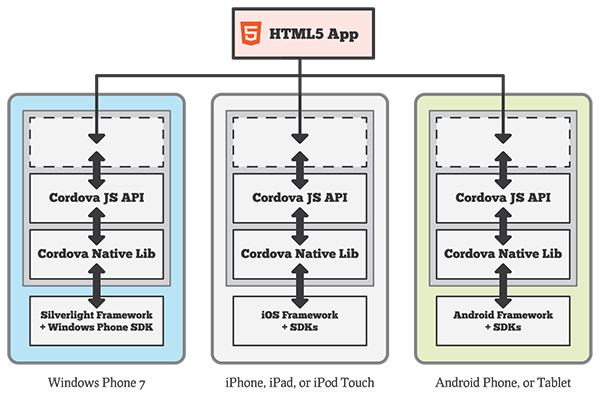
\includegraphics[scale=0.6]{html5app.png}
\caption{Ứng dụng HTML5}
\end{figure}

Cordova cũng có thể được mở rộng với nguồn gốc của các plug-in cho phép các nhà phát triển thêm các chức năng có thể được gọi từ JavaScript, cho phép giao tiếp trực tiếp giữa các lớp bản địa và các trang HTML5. Cordova bao gồm bổ sung cơ bản cho phép truy cập vào gia tốc của thiết bị, camera, microphone, la bàn, hệ thống tập tin, và nhiều hơn nữa.

Tuy nhiên, việc sử dụng công nghệ web dựa trên dẫn nhiều ứng dụng Cordova để chạy chậm hơn so với các ứng dụng bản địa với chức năng tương tự. Adobe Systems cảnh báo rằng các ứng dụng được xây dựng sử dụng Cordova có thể bị từ chối bởi của Apple là quá chậm hoặc không cảm thấy "bản địa" đủ (có sự xuất hiện và chức năng phù hợp với những gì người dùng đã mong đợi trên nền tảng này).

\subsection{Nền tảng ứng dụng di động Worklight}

IBM Worklight cung cấp một nền tảng ứng dụng di động cao cấp, toàn diện và mở, có thể giúp phát triển, chạy và quản lý có hiệu quả các ứng dụng HTML5, lai và nguyên gốc, bằng cách sử dụng các công nghệ và các công cụ dựa trên các tiêu chuẩn, phần mềm trung gian tối ưu hóa cho di động, một loạt các cơ chế bảo mật và các khả năng phân tích và quản lý tích hợp.

\begin{figure}[!htb] 
\centering
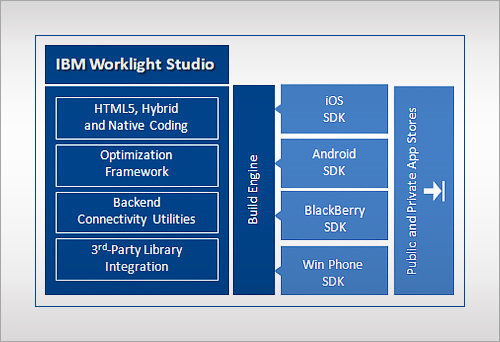
\includegraphics[scale=0.6]{worklight_eco.png}
\caption{Nền tảng ứng dụng di động Worklight}
\end{figure}

Worklight giúp xây dựng các ứng dụng lai (hybrid), bổ sung những khiếm khuyết của ứng dụng nền web như không can thiệp sâu vào thiết bị hay không khởi chạy được các thành phần đa phương tiện bằng những phương thức của ứng dụng nguyên bản (native).

Đề tài được ứng dụng trên phiên bản Worklight 6 của IBM.

\subsection{Truyền thông qua Web services}
\subsubsection{Tổng quan về Web services}

Web services là kiến trúc hỗ trợ khả năng tương tác của các ứng dụng trên các máy tính khác nhau thông qua mạng Internet với giao diện chung và sự gắn kết được mô tả bằng XML và truy xuất thông qua web dùng URL.

Lợi điểm của Web services là chi phí phát triển thấp, dễ bảo trì, cho phép Client và Server tương tác được với nhau trong những môi trường khác nhau.

Web services là một dịch vụ cung cấp cơ chế triệu gọi các đối tượng từ xa thông qua giao thức HTTP cùng với cơ chế truyền tải định dạng đối tượng theo công nghệ XML. Chính vì sử dụng giao thức HTTP của Web nên giờ đây các lời gọi trở nên đơn giản và thông qua được các rào cản về tường lửa. Để đảm bảo điều này, một giao thức mới là SOAP (Simple Object Access Protocol) ra đời để hỗ trợ cho Web services.  

\textbf{SOAP – Simple Object Access Protocol}

SOAP được định nghĩa dựa trên giao thức chuẩn HTTP, SOAP cho phép dữ liệu chuyển đi bằng HTTP và định dạng theo chuẩn XML. Các lời gọi hàm tham số truyền hàm, dữ liệu trả về từ hàm, tất cả đều được chuyển sang dạng XML và có thể dễ dàng xử lý bởi tất cả các ngôn ngữ. Một thế mạnh khác đó là nếu các đối tượng phân tán xây dựng trên mô hình Web services sẽ có thể triệu gọi lẫn nhau, bất chấp đối tượng đó được viết trên ngôn ngữ Java của Sun hay .NET của Microsoft.
  
Hiện tại, SOAP được coi là một sự thay đổi lớn kể từ khi COM, RMI, CORBA ra đời.

\subsubsection{Đặc điểm web services}

\textbf{Độc lập ngôn ngữ:}

Web services được truy xuất thông qua Web bằng cách dùng URL.

Web services liên lạc với thế giới bên ngoài dùng thông điệp XML gửi trực tiếp qua các giao thức Web.

Web services được đăng ký tại nơi chung, và được đặc tả tất cả các chức năng.

\textbf{Chi phí phát triển thấp, dễ bảo trì.}

Dịch vụ Web cho phép client và server tương tác được với nhau ngay cả trong những môi trường khác nhau. Ví dụ, đặt Web server cho ứng dụng trên một máy chủ chạy hệ điều hành Linux trong khi người dùng sử dụng máy tính chạy hệ điều hành Windows, ứng dụng vẫn có thể chạy và xử lý bình thường mà không cần thêm yêu cầu đặc biệt để tương thích giữa hai hệ điều hành này.

Phần lớn kĩ thuật của Dịch vụ Web được xây dựng dựa trên mã nguồn mở và được phát triển từ các chuẩn đã được công nhận, ví dụ như XML.

Một Dịch vụ Web bao gồm có nhiều mô-đun và có thể công bố lên mạng Internet.

Là sự kết hợp của việc phát triển theo hướng từng thành phần với những lĩnh vực cụ thể và cơ sở hạ tầng Web, đưa ra những lợi ích cho cả doanh nghiệp, khách hàng, những nhà cung cấp khác và cả những cá nhân thông qua mạng Internet.

Một ứng dụng khi được triển khai sẽ hoạt động theo mô hình client-server. Nó có thể được triển khai bởi một phần mềm ứng dụng phía server ví dụ như PHP, Oracle Application server hay Microsoft.Net…

Ngày nay dịch vụ Web đang rất phát triển, những lĩnh vực trong cuộc sống có thể áp dụng và tích hợp dịch vụ Web là khá rộng lớn như dịch vụ chọn lọc và phân loại tin tức (hệ thống thư viện có kết nối đến web portal để tìm kiếm các thông tin cần thiết); ứng dụng cho các dịch vụ du lịch (cung cấp giá vé, thông tin về địa điểm…), các đại lý bán hàng qua mạng, thông tin thương mại như giá cả, tỷ giá hối đoái, đấu giá qua mạng…hay dịch vụ giao dịch trực tuyến (cho cả B2B và B2C) như đặt vé máy bay, thông tin thuê xe…

Các ứng dụng có tích hợp dịch vụ Web đã không còn là xa lạ, đặc biệt trong điều kiện thương mại điện tử đang bùng nổ và phát triển không ngừng cùng với sự lớn mạnh của Internet. Bất kì một lĩnh vực nào trong cuộc sống cũng có thể tích hợp với dịch vụ Web, đây là cách thức kinh doanh và làm việc có hiệu quả bởi thời đại ngày nay là thời đại của truyền thông và trao đổi thông tin qua mạng. Do vậy, việc phát triển và tích hợp các ứng dụng với dịch vụ Web đang được quan tâm phát triển là điều hoàn toàn dễ hiểu.

\section{Khảo sát}

Nhìn chung lĩnh vực E-learning trên tablet cũng khá nổi trong những năm gần đây, khi mà giá thành chiếc tablet ngày càng rẻ, hơn nữa tablet sẽ dễ dàng sử dụng hơn là laptop hay desktop. Một trong những phần mềm học tiếng Anh mà chúng em đã khảo sát sau đây khá điển hình. Phần mềm luyện nghe tiếng anh thường chỉ chạy trên một nền tảng nhất định, trong trường hợp này là viết bằng Java chạy trên hệ điều hành Android. Trong khi đó phần mềm mà chúng em viết bằng JavaScript, và chỉnh cần tinh chỉnh một chút là có thể chạy cả trên Android hay iOS.
\subsection{IELTS Listening}

\begin{figure}[!htb] 
\centering
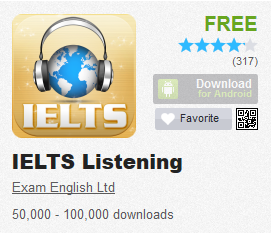
\includegraphics[scale=0.8]{iel.png}
\caption{Chương trình IELTS Listening trên Android}
\end{figure}

Chương trình luyện nghe IELTS miễn phí chạy trên Android với lượt download là 50,000-100,000:

Đường dẫn đến website \url{http://www.appszoom.com/android_applications/education/ielts-listening_hddku.html}

\begin{figure}[!htb] 
\centering
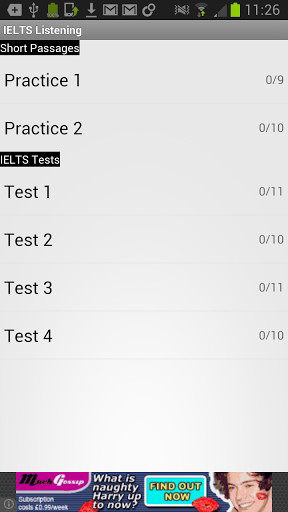
\includegraphics[scale=0.4]{iel1.png}

\caption{Màn hình chọn bài học của chương trình}
\end{figure}

\begin{figure}[!h] 
\centering
\subfigure[Màn hình trả lời trắc nghiệm]{
   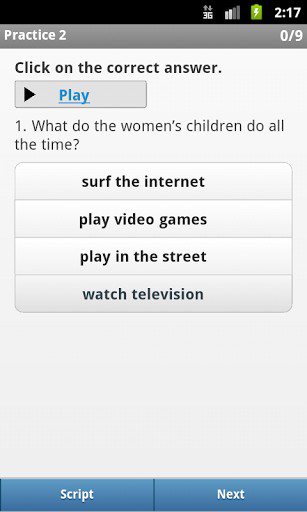
\includegraphics[width=0.30\textwidth] {iel2.png}
   \label{fig:MultipleChoices}}
\subfigure[Màn hình điền từ vào chỗ trống]{
   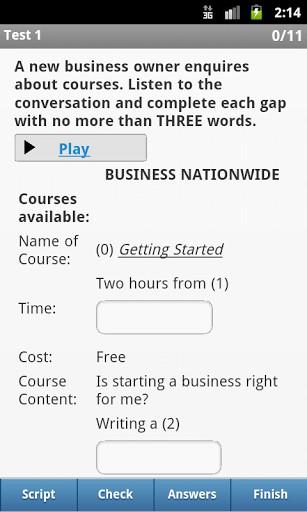
\includegraphics[width=0.30\textwidth] {iel3.png}
   \label{fig:Fillblank}}

\caption{Màn hình chính của chương trình }
\end{figure}




\subsection{English Ant plus}

English Ant plus (Bản office): Phần mềm học tiếng anh trên android

Giao diện đơn giản, dễ nhìn.

\begin{figure}[!htb] 
\centering
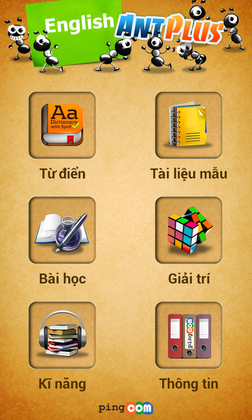
\includegraphics[scale=0.8]{hinh1_menu.png}
\caption{Màn hình menu của chương trình}
\end{figure}

Phần mềm có các chức năng chính như sau:

\quad 1. Từ điển

Chức năng Từ điển cũng tương tự như các từ điển thông dụng.


Khi đánh một từ thì 1 danh sách từ được đề nghị xổ xuống.

Có từ điển chuyên ngành về kỹ thuật và kinh tế.

\quad 2. Tài liệu mẫu

Có một thư viện mẫu về Thư giao dịch, Sơ yếu lý lịch và Hợp đồng mẫu bằng Tiếng Anh.

Mỗi một mục phân ra làm nhiều lĩnh vực, ngành nghề khác thuận tiện trong việc tìm kiếm.

Đa số các lĩnh vực phổ biến nó đều có như: thư giao dịch trong ngân hàng, mua bán, các hợp đồng làm ăn…

\quad 3. Bài học

Chứa các bài học về ngữ pháp, từ vựng.

Có hầu hết các chủ đề phổ biến.

Hỗ trợ update dữ liệu mới về và hỗ trợ tìm kiếm chủ đề mình muốn học.

\quad 4. Trò chơi

Vừa học vừa chơi.

Có 3 trò chơi là: Thách thức, Ô chữ và Treo cổ.

\quad 5. Kỹ năng

Luyện kĩ năng nghe và đọc hiểu của mình.

Có 2 lựa chọn là karaoke và VOA Special English.

Phần karaoke gần 100 bài hát tiếng Anh hay, bất hủ.

Phần VOA Special English có khá nhiều bài viết bằng tiếng Anh theo nhiều chủ đề khác nhau.

Phần đọc hiểu cũng cung cấp khá nhiều bài. Có thể cập nhật lại cơ sở dữ liệu, từ server của PINGCOM.

Phần bài luận: Cung cấp cho người dùng rất nhiều bài luận về nhiều vấn đề, và những quan điểm về các vấn đề đó. Từ những bài luận này mình có thể học được cách viết bài, viết báo cáo...


\begin{figure}[!h] 
\centering
\subfigure[Màn hình từ điển]{
   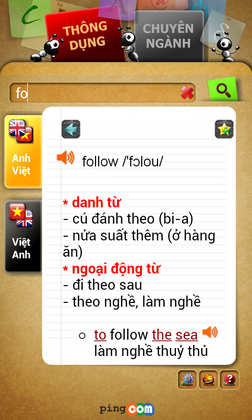
\includegraphics[width=0.30\textwidth] {hinh2_dist.png}
   \label{fig:Dict}}
\subfigure[Màn hình tài liệu]{
   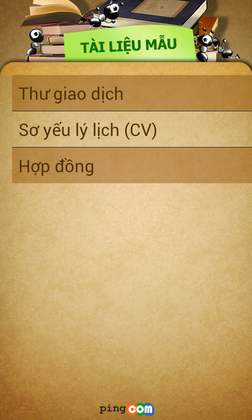
\includegraphics[width=0.30\textwidth] {hinh3_doc.png}
   \label{fig:Doc}}
\subfigure[Màn hình bài học]{
   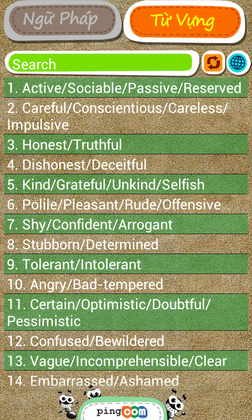
\includegraphics[width=0.30\textwidth] {hinh4_lesson.png}
   \label{fig:Lession}}
\subfigure[Màn hình luyện kĩ năng nghe và đọc]{
   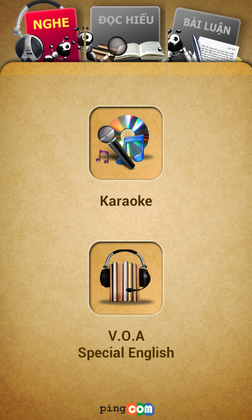
\includegraphics[width=0.30\textwidth] {hinh6_skills.png}
   \label{fig:Skill}}
\caption{Màn hình chính của chương trình }
\end{figure}

\subsection{Nhận xét chung}

Đa phần các phần mềm luyện nghe nói riêng và học tiếng Anh nói chung ở trên đều chỉ chạy ở một nền tảng nhất định, không có chức năng kết nối mạng để cập nhật nội dung bài học.

\section{Tổng kết chương}

Đa phần các chương trình luyện nghe tiếng Anh nói riêng và luyện học ngoại ngữ nói chung trên tablet thường chỉ chạy trên một nền tảng nhất định nào đó và thường là dạng ứng dụng offline. Còn đối với ứng dụng mà chúng em nghiên cứu và hiện thực sẽ có thể chạy trên nhiều nền tảng hệ điều hành khác nhau, và với sự hỗ trợ mạnh mẽ từ Moodle, sẽ giúp cho giáo viên soạn bài học được tốt hơn, tương tác với học viên tốt hơn, do ứng dụng chúng em cần phải có kết nối Internet để giảng viên có thể đổi nội dung bài học hay câu hỏi bất cứ lúc nào cũng được và ứng dụng trên tablet sẽ phải theo đó và hiện lên nội dung mới nhất mà giáo viên thay đổi, góp phần tạo nên sự tương tác giữa dạy và học, giữa giáo viên và học viên.